%%% template.tex
%%%
%%% This LaTeX source document can be used as the basis for your technical
%%% paper or abstract. Intentionally stripped of annotation, the parameters
%%% and commands should be adjusted for your particular paper - title,
%%% author, article DOI, etc.
%%% The accompanying ``template.annotated.tex'' provides copious annotation
%%% for the commands and parameters found in the source document. (The code
%%% is identical in ``template.tex'' and ``template.annotated.tex.'')

\documentclass[]{acmsiggraph}
\usepackage{algorithm}
\usepackage[noend]{algpseudocode}
\TOGonlineid{45678}
\TOGvolume{0}
\TOGnumber{0}
\TOGarticleDOI{0}
\TOGprojectURL{}
\TOGvideoURL{}
\TOGdataURL{}
\TOGcodeURL{}
\usepackage{color}
%\definecolor{red}{rgb}{0.9, 0.17, 0.31}
\usepackage{multirow}
\usepackage{subfig}
\usepackage{xcolor}
\usepackage{lipsum}
\usepackage{listings}
\usepackage{graphicx}
\usepackage{glsllst} % My own package providing markup listing for glsl
\usepackage{rmlst}   % My own package providing markup listing for renderman
\usepackage{amsmath}
\usepackage{hyperref}

\lstset{
backgroundcolor=\color[rgb]{0.95, 0.95, 0.95},
tabsize=3,
	%rulecolor=,
	basicstyle=\footnotesize\ttfamily,
	upquote=true,
	aboveskip={1.5\baselineskip},
	columns=fixed,
	showstringspaces=false,
	extendedchars=true,
	breaklines=true,
	prebreak = \raisebox{0ex}[0ex][0ex]{\ensuremath{\hookleftarrow}},
	frame=none,
	aboveskip=15pt,
	belowskip=8pt,
	captionpos=t,
	showtabs=false,
	showspaces=false,
	showstringspaces=false,
	identifierstyle=\ttfamily,
	%keywordstyle=\color{red}\bfseries,
	%keywordstyle=[1]\bfseries\color{syntaxBlue},
	%keywordstyle=[2]\bfseries\color{syntaxRed},
	%keywordstyle=[3]\color{blue}\bfseries,
	%keywordstyle=[4]\bfseries\color{syntaxBlue},
	commentstyle=\color[rgb]{0.082,0.639,0.082},
	keywordstyle=[1]\bfseries\color[rgb]{0,0,0.75},
	keywordstyle=[2]\bfseries\color[rgb]{0.5,0.0,0.0},
	keywordstyle=[3]\bfseries\color[rgb]{0.127,0.427,0.514},
	keywordstyle=[4]\bfseries\color[rgb]{0.4,0.4,0.4},
	stringstyle=\color[rgb]{0.639,0.082,0.082},
	}

	\title{Masterclass Assignment: Real-time Global Illumination}

	\author{Joe Withers\thanks{e-mail: joewithers96@gmail.com}}
	\pdfauthor{Joe Withers}

	\keywords{rendering}

	\begin{document}

%% \teaser{
%%   \includegraphics[height=1.5in]{images/sampleteaser}
%%   \caption{Spring Training 2009, Peoria, AZ.}
%% }

\maketitle

\begin{abstract}
This document details the approach I took to complete the Masterclass assignment, evaluates the results, and lists possible improvements I could make in the future.
\end{abstract}
%\keywordlist
%\TOGlinkslist

\section{Introduction}
For this assignment I decided to implement the technique \textit{Interactive Indirect Illumination using voxel cone tracing} \cite{crassinneyretsainzgreeneisemann2011}, commonly referred to as VXGI, to achieve realtime global illumination. This technique achieves real-time global illumination rendering the directly illuminated scene geometry into a three-dimensional texture, which can be sampled in a deferred shading pass using cone tracing to calculate accurate indirect diffuse and specular lighting terms.

\section{Method}
I used C++ and OpenGL for this assignment, utilising the NCCA Graphics Library NGL \cite{ngl} to interact with OpenGL, and Qt5 to create the user interface. I based my implementation around a demo of the Sponza atrium using NGL \cite{pbrSponza}, that although is quite old, saved me from spending a lot of time writing a grouped Wavefront OBJ and MTL file parser. I extended upon this demo by converting it to use deferred shading, which is necessary for VXGI and other post process effects, using tutorial material from LearnOpenGL \cite{learnDeferred}.

The first step of implementing VXGI was to create a voxelized representation of the albedo and surface normal information in the scene. The method used in the source material \cite{crassinneyretsainzgreeneisemann2011} is explained in great detail in an OpenGL Insights chapter titled \textit{Octree-Based Sparse Voxelization Using the GPU Hardware Rasterizer} \cite{crassingreen2012}, but the basic concept is as followed:
\begin{enumerate}
	\item Generate three projection matrices for orthogonal projections, covering the scene geometry equally, and aligned to each of the coordinate axes.
	\item Draw the scene with depth testing disabled, ensuring fragments are generated for every triangle.
	\item For each triangle, determine which of the coordinate axes is most aligned with the surface normal, thus generating the maximum number of fragments when transformed using the corresponding projection matrix for that axis.
	\item Using either the NVIDIA OpenGL extension \textit{GL CONSERVATIVE RASTERIZATION NV}, or a geometry shader, enlarge each triangle so that fragments are generated regardless of whether it covers a pixels center. This helps to reduce 'cracks' in the voxelisation on surfaces that are angled away from the coordinate axes.
	\item Using the fragment coordinates, depth, and the axis chosen in step 3, infer the texel coordinate that the fragment corresponds to in the target 3D textures. Store the fragment albedo and normal information in 3D textures using a moving average.
\end{enumerate}
Whilst this technique is somewhat easy to explain, I had not previously used the required Image Load/Store commands so I referred to an implementation I found on GitHub \cite{voxelization} to guide me on the OpenGL side of things.

The next step was to inject the scene's emissive values into a 3D texture. This is achieved by raytracing towards the light, for each of the non-transparent texels in the voxelised textures. This is where my implementation differs from the source material \cite{crassinneyretsainzgreeneisemann2011} as I opted to use a dense 3D texture as opposed to a sparse voxel octree. Whilst this was significantly easier to set up, it also severly impacts the speed at which raytracing can be performed through this 3D texture (See Figure~\ref{figure:performance} for performance metrics). The source material \cite{crassinneyretsainzgreeneisemann2011} also details a method for mip-mapping this texture anisotropically along each of the coordinate axes, however I opted to use OpenGL's \lstinline{genMipMaps} method to save time.

The final step was to implement cone tracing in the deferred shading pass. This pass calculates the indirect light contribution, specular lobe contribution, and also soft shadows, using the emissive 3D texture and the textures generated by the G-Buffer.

\begin{figure}[htbp]\centering
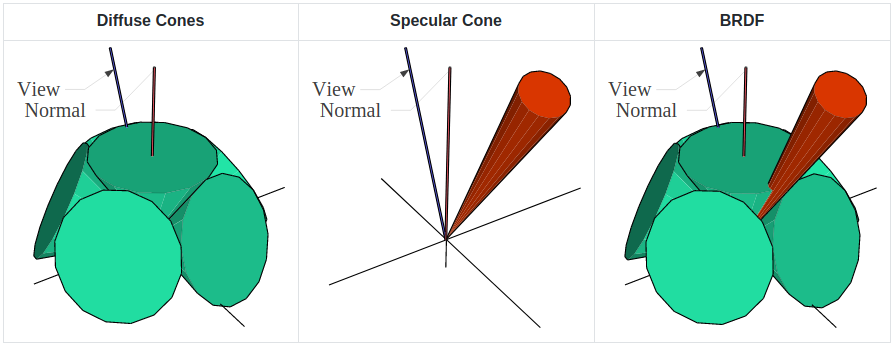
\includegraphics[width=1.0\linewidth]{images/BRDF}
\caption{\label{figure:BRDF} A series of diagrams showing how the combination of a specular cone and multiple diffuse cones can be used to approximate a material BRDF. \protect\cite{Villegas2016} The diffuse cones form a normal-oriented hemisphere to approximate the diffuse reflections, whilst the specular cone follows the reflection vector and it's aperture varies dependent on the material roughness.}
\end{figure}

For the indirect and specular light contributions I referred to VCTRenderer \cite{Villegas2016} for example code on implementing an efficient cone tracing function, and how it can be used to approximate a BRDF as shown in Figure~\ref{figure:BRDF}. I then adapted the specular component to work with the PBR materials to ensure the specular cone aperture is physically plausible for any given viewing angle.

To calculate the the direct lighting contribution I referred to tutorial materian from LearnOpenGL \cite{learnPBR} to ensure that the PBR textures passed through the G-Buffer are combined in a physically plausible way. I referred again to VCTRenderer \cite{Villegas2016} to implement soft shadows into the direct lighting component, which involves calculating a fragment's occlusion by tracing a cone back towards the light source and accumulating the opacity values at each step.

Finally I added additional controls to the interface and passed them as uniforms to the deferred shading pass, allowing the user to control the following parameters:
\begin{itemize}
	\item The overall contributions of each lighting component.
	\item Whether to enable or disable the calculation of each lighting component, as shown in Figures~\ref{figure:direct},~\ref{figure:indirect},~\ref{figure:specular}.
	\item The cone aperture for tracing the soft shadows. Larger values can be used to estimate larger light sources.
	\item The light falloff exponent $k$ relative to the $distance$ to the light. Light falloff is calculated as $1 / (distance^k)$, so the default value of 2.0 is physically plausible.
	\item A multiplier for the specular cone aperture. Smaller values can make the scene highly reflective as shown in Figure~\ref{figure:reflection}.
\end{itemize}

\section{Results}

Figure~\ref{figure:fullrender} shows a series of screenshots of my final results with all of the lighting passes enabled. Whilst I am pleased with the outcome, there are also a number of visual artefacts that I discuss in Section~\ref{section:improvements}. Figure~\ref{figure:performance} shows some performance metrics for the individual lighting passes at different voxel resolutions. Note that memory usage is high, even at low resolutions, as I opted to use dense 3D textures as opposed to sparse 3D textures. The time taken to perform the light injection pass also scales quite poorly at high resolutions because of this. Despite this, moving around the scene maintains a smooth 60 frames per second (limited by the OpenGL context), providing the user does not move the light. The voxelization and shading passes seem to scale very well with increased resolution, taking on average 2 and 4.5 miliseconds respectively at all of the tested resolutions.

\begin{figure}[htbp]\centering
\begin{center}
\begin{tabular}{|c|c|c|c|}
\hline
Voxel Resolution & $256^3$ & $512^3$ & $768^3$ \\
\hline
\hline
Frames per second & 60 & 60 & 60 \\
\hline
Memory usage & 1063MiB & 2615MiB & 6628MiB \\
\hline
Voxelization & 2ms & 2ms & 2ms \\
\hline
Light Injection & 65ms & 378.5ms & 12294.5ms\\
\hline
Shading & 4.5ms & 4.5ms & 4.5ms \\
\hline
\end{tabular}
\caption{\label{figure:performance} Averaged performance results when running with a NVIDIA GTX 1080 8GB at 2560x1080.}
\end{center}
\end{figure}
\begin{figure}[htbp]\centering
\includegraphics[width=1.0\linewidth]{images/full_render_01}
\includegraphics[width=1.0\linewidth]{images/full_render_02}
\includegraphics[width=1.0\linewidth]{images/full_render_03}
\caption{\label{figure:fullrender}Three screenshots showing the full scene with a voxel resolution of $512^3$.}
\end{figure}
\begin{figure}[htbp]\centering
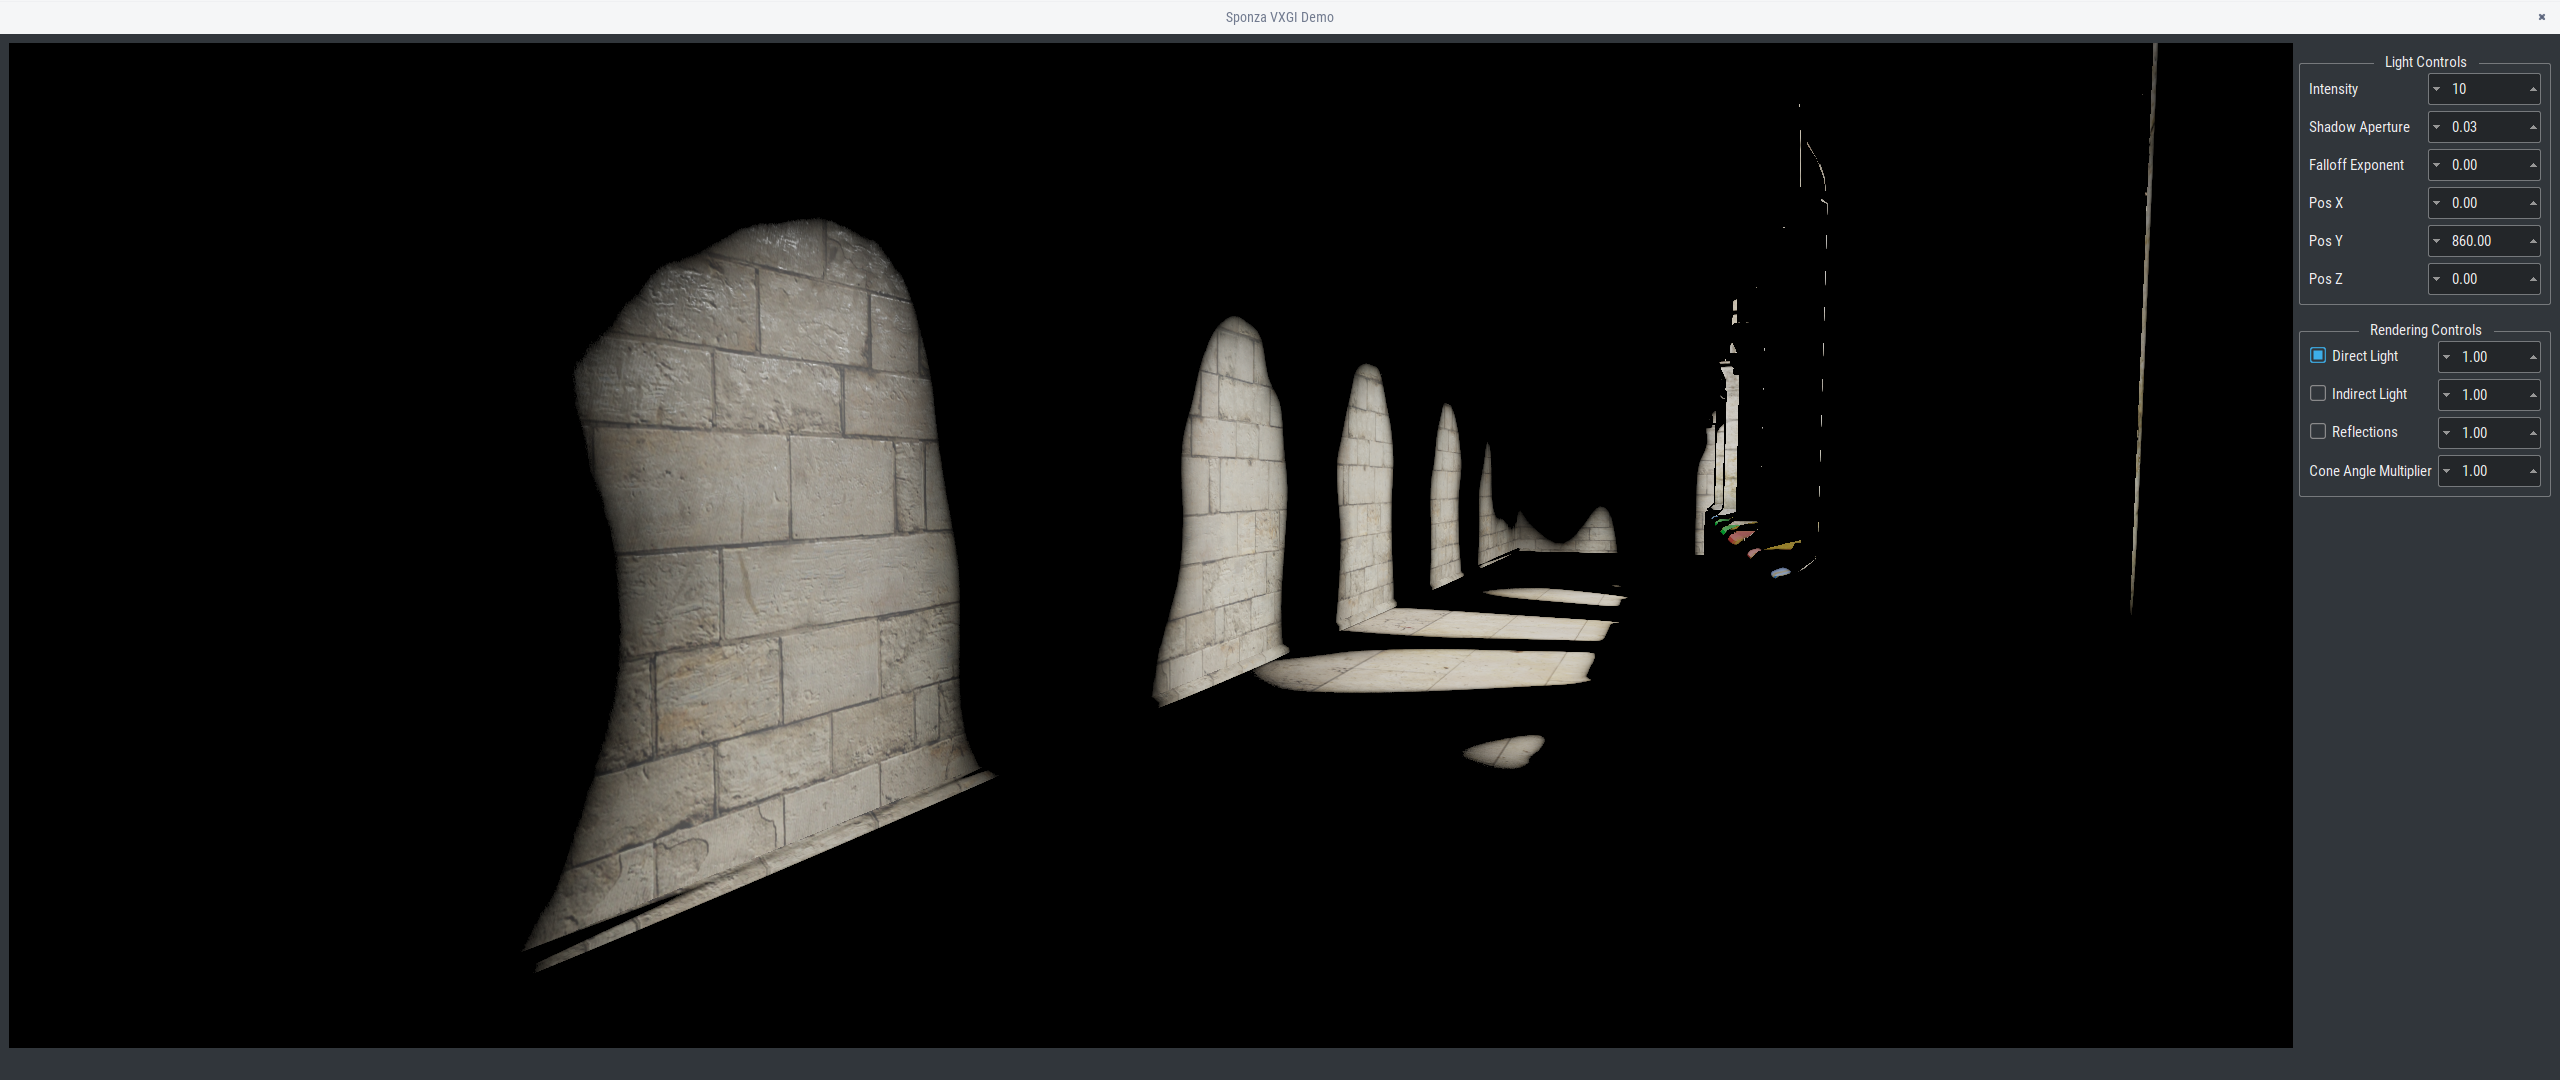
\includegraphics[width=1.0\linewidth]{images/direct_only}
\caption{\label{figure:direct}A screenshot showing just the direct lighting component.}
\end{figure}
\begin{figure}[htbp]\centering
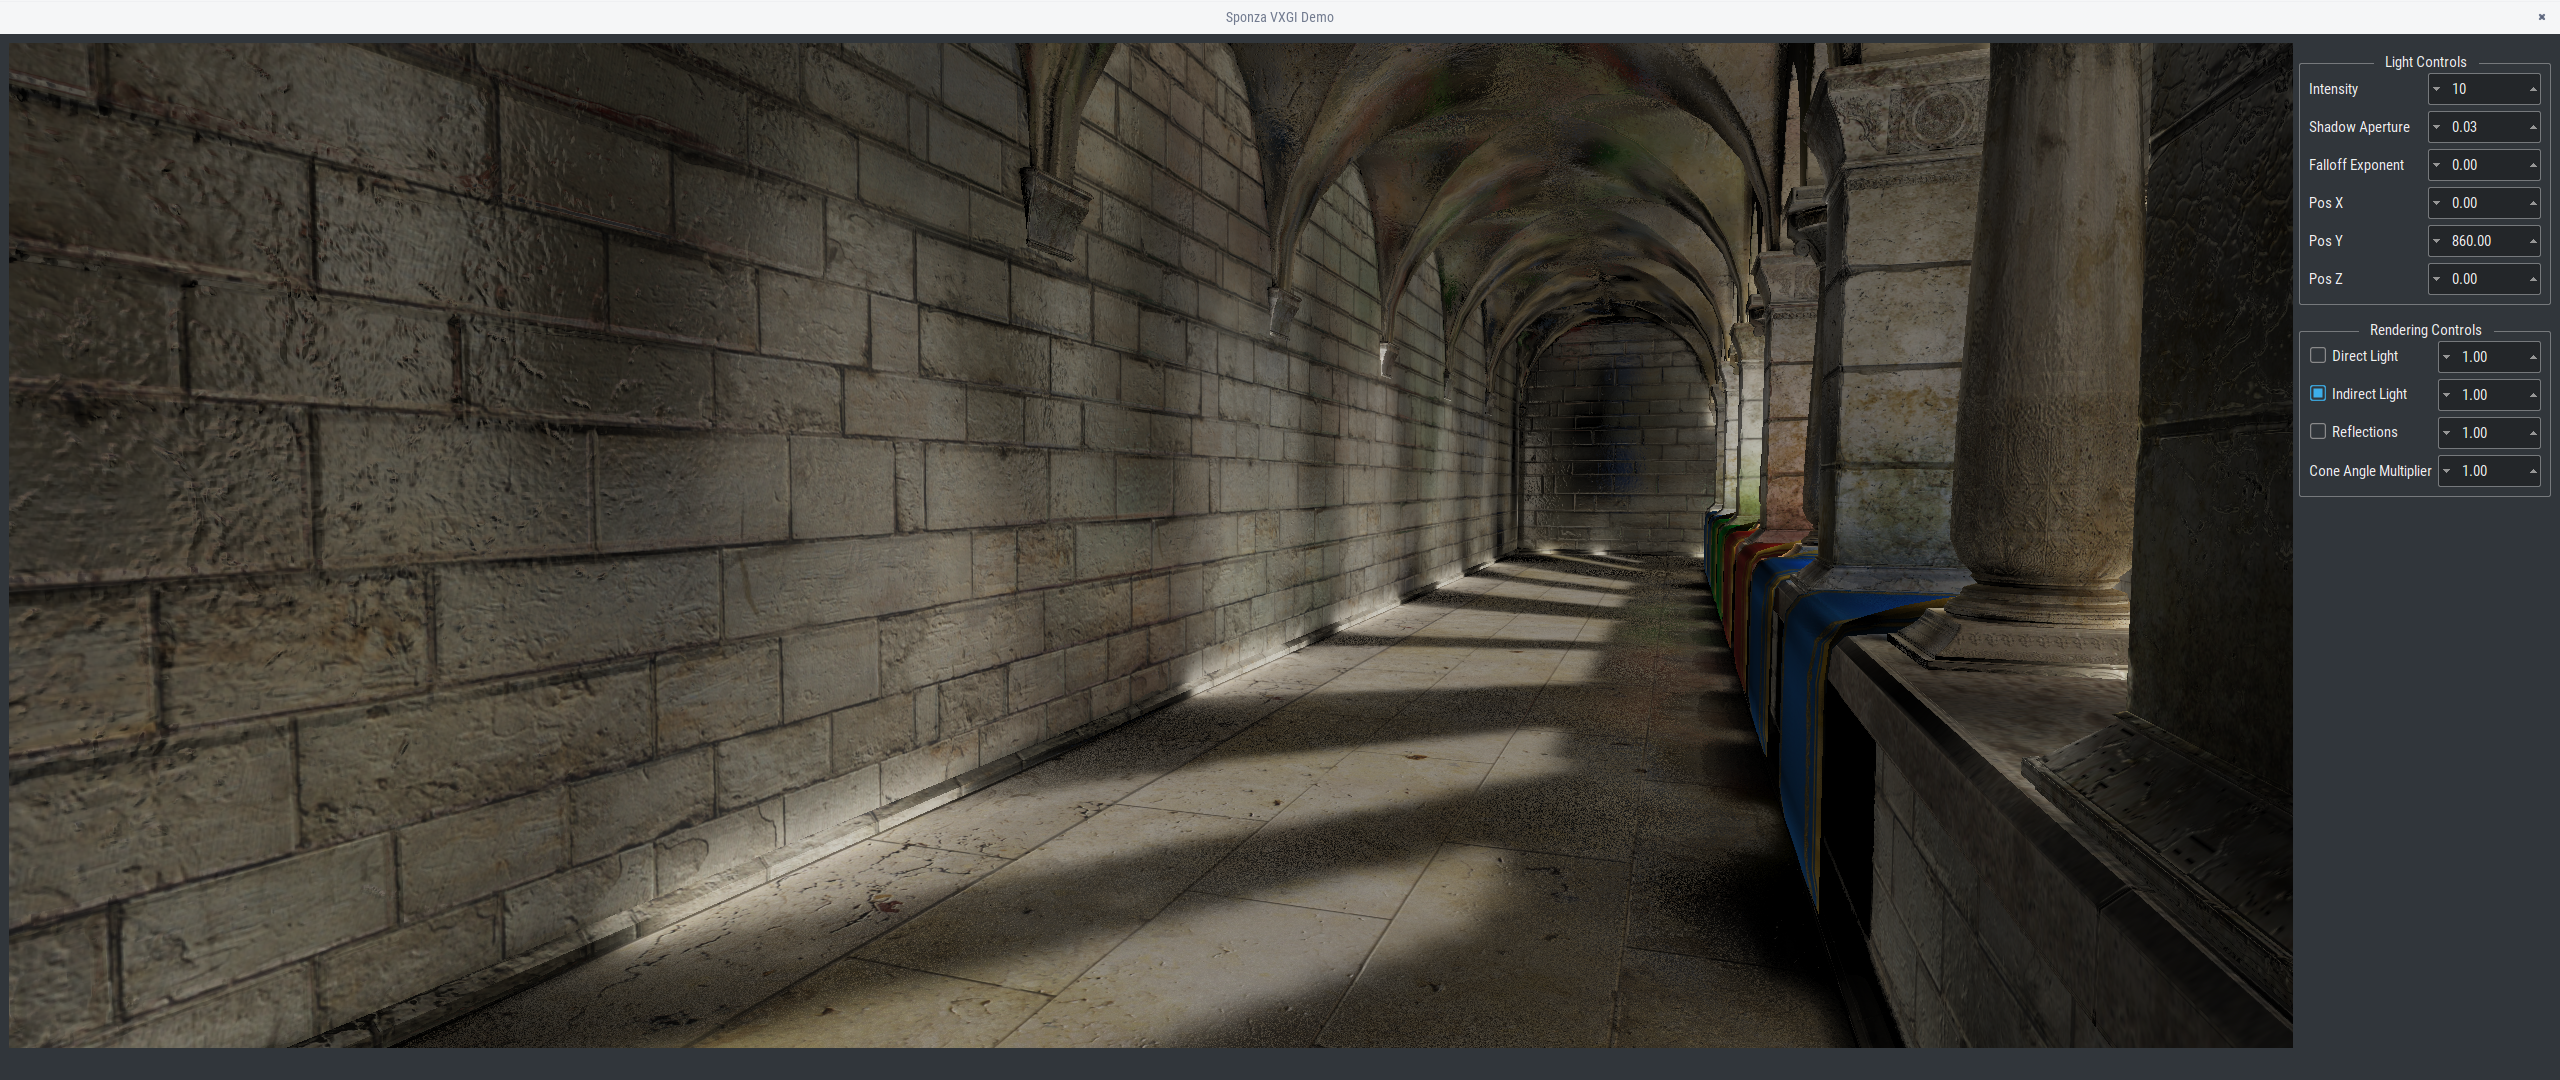
\includegraphics[width=1.0\linewidth]{images/indirect_only}
\caption{\label{figure:indirect}A screenshot showing just the indirect lighting component.}
\end{figure}
\begin{figure}[htbp]\centering
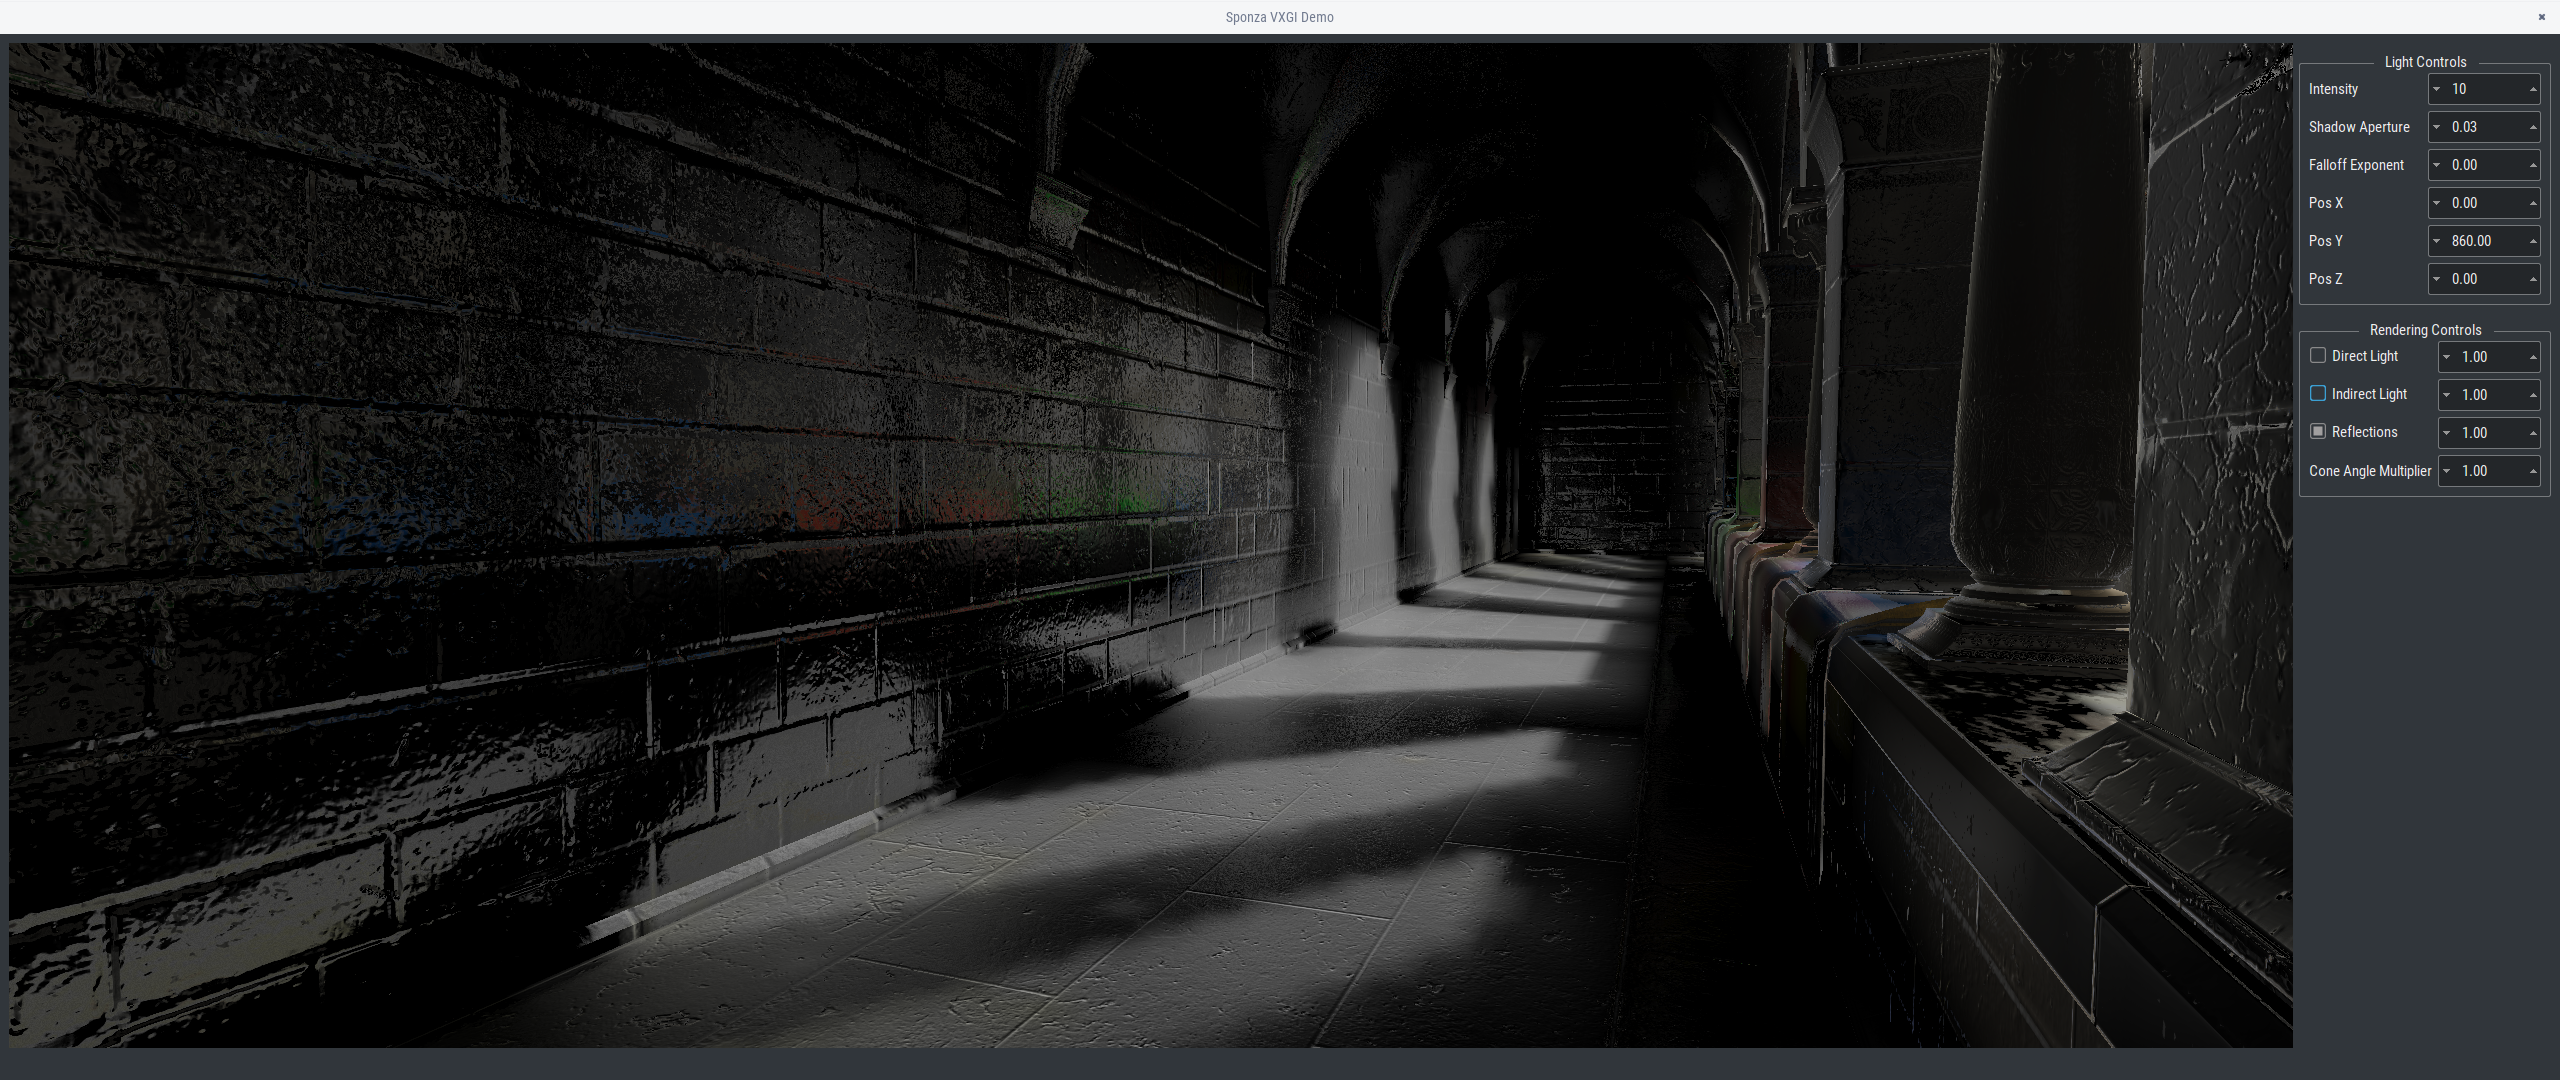
\includegraphics[width=1.0\linewidth]{images/reflection_only}
\caption{\label{figure:specular}A screenshot showing just the specular component.}
\end{figure}
\begin{figure}[htbp]\centering
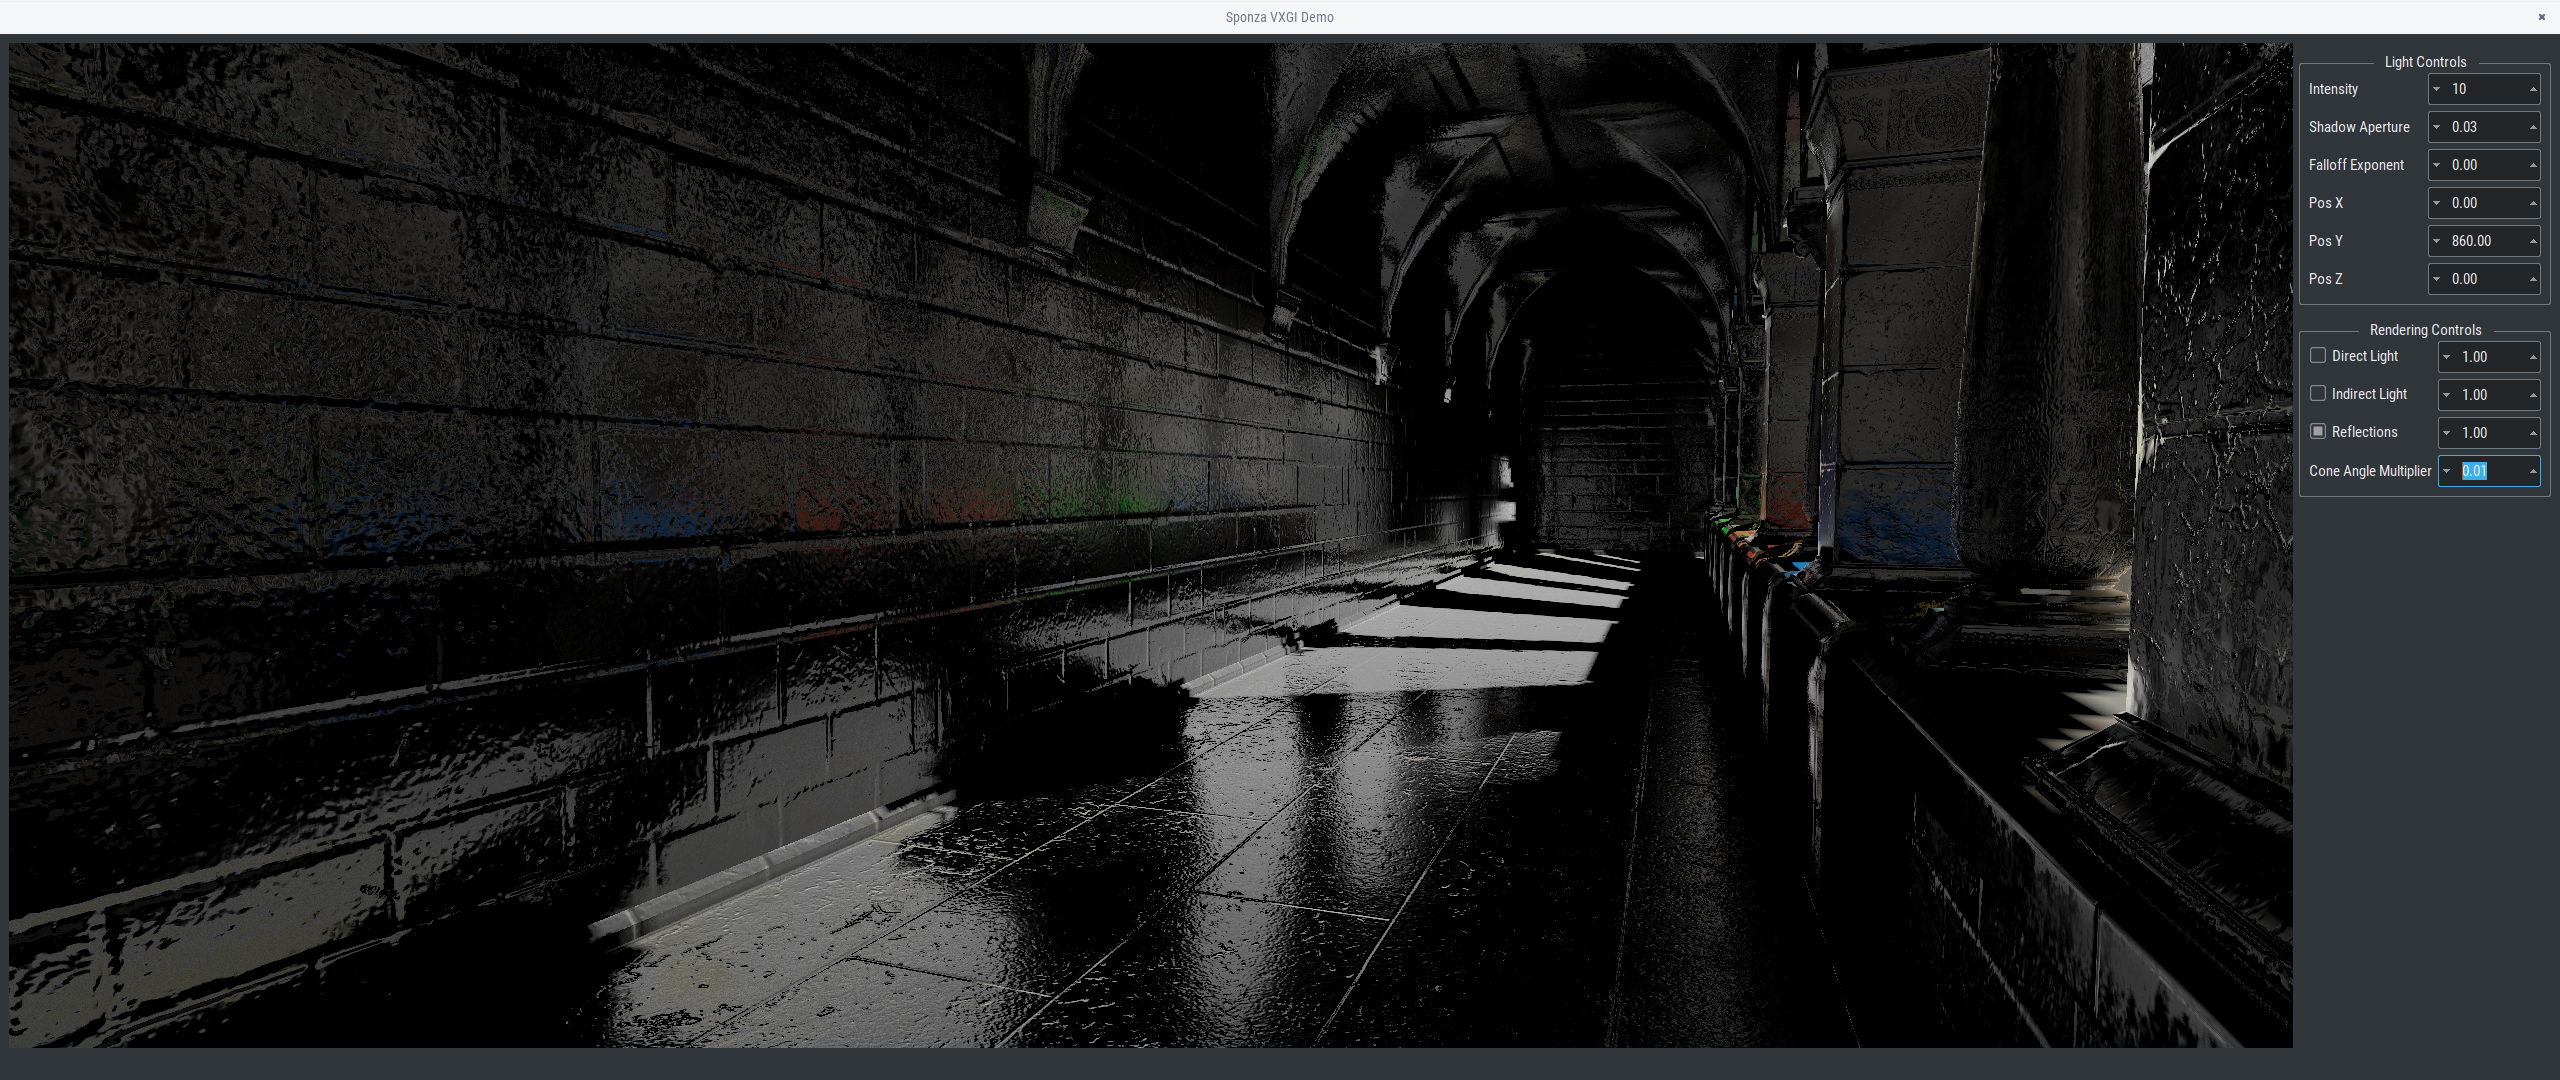
\includegraphics[width=1.0\linewidth]{images/reflection_only_no_roughness}
\caption{\label{figure:reflection}A screenshot showing just the specular component, but with the minimum cone aperture.}
\end{figure}

\section{Future Improvements} \label{section:improvements}

Unfortunately I wasn't able to implement a sparse data structure as described in the source material \cite{crassinneyretsainzgreeneisemann2011} before the assignment deadline. Having a sparse data structure to store the emissive voxel texture would save a significant amount of GPU memory consumption, allowing the resolution for voxelization to be much higher; currently with dense 3D textures it is capable of exceeding both the 2 gigabyte memory limit of my GPU, and the 8 gigabyte limit of those at university.

The speed at which lighting rays are marched during the light injection pass would also be improved, as it would be able to step further through the voxel texture whilst ray marching if the higher levels in the octree are known to be empty.

I did start working on a sparse voxel octree as described in OpenGL Insights \cite{crassingreen2012} by using an OpenGL Atomic Counter for calculating the number of fragments needed for the voxel fragment list, and I believe I understand the technique well enough should I wish to implement it in the future.

The source material \cite{crassinneyretsainzgreeneisemann2011} also describes a method for anisotropic mip-mapping of the 3D texture, storing a version of the texture for each directional axis, which improves visual accuracy when cone tracing. Whilst I could have implemented this with the dense 3D textures I was using, I opted to use OpenGL's built in mip-mapping to save time.

There are also a number of visual artefacts, the most noticable of which being the cracks in the voxelization as seen in Figure~\ref{figure:cracks}. I understand this to be due to incorrect conservative rasterization, however I have the NVIDIA \textit{GL CONSERVATIVE RASTERIZATION NV} extension enabled and have confirmed it to be working, so I believe it could be an issue with using the extension whilst having multisampling enabled (as it is currently). I found that using a geometry shader to achieve the same result led to quite unusable artefacting.

Another artefact is quite visible noise in the indirect lighting component, as seen in Figure~\ref{figure:noise}. I am not sure what causes this, though I suspect it could be because the hemisphere of indirect cones are aligned with the normal-mapped surface normal as opposed to the surface normal recieved from the geometry, which results in excessive variance between indirect lighting calculations for neighboring fragments. Banding artefacts are visible in the specular component, as seen in Figure~\ref{figure:banding}, which occurs at certain viewing angles and at certain values for the specular aperture multiplier. I suspect this is a combination of excessive variance in surface normals, as mentioned previously, but could also be a result of limited numerical precision in calculating the specular component.

\begin{figure}[htbp]\centering
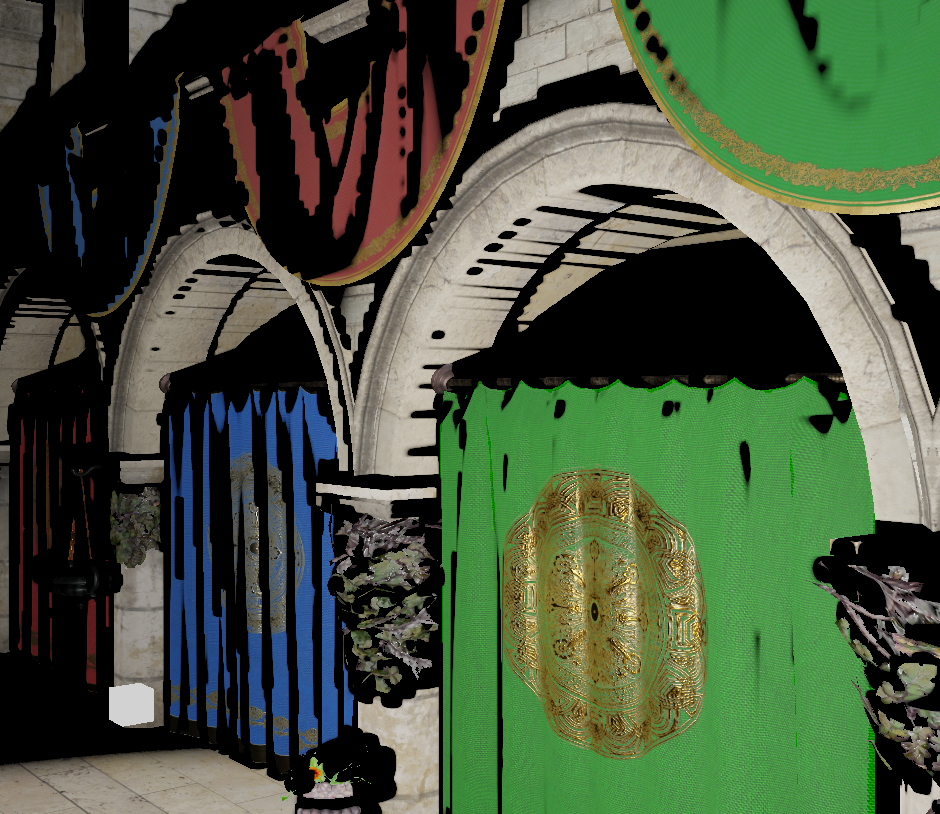
\includegraphics[width=1.0\linewidth]{images/voxelization_error.png}
\caption{\label{figure:cracks}A screenshot showing voxelization artefacts.}
\end{figure}
\begin{figure}[htbp]\centering
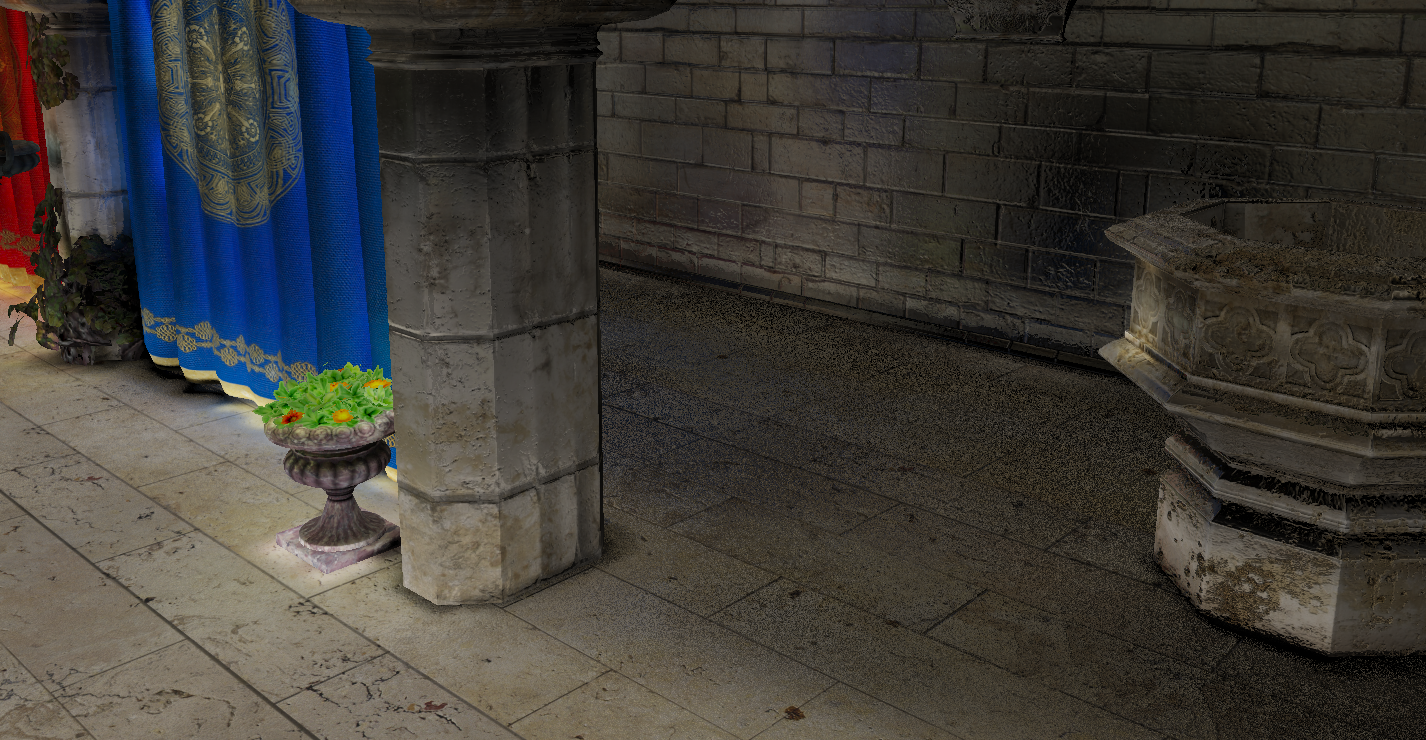
\includegraphics[width=1.0\linewidth]{images/indirect_noise.png}
\caption{\label{figure:noise}A screenshot showing noise in the indirect lighting.}
\end{figure}
\begin{figure}[htbp]\centering
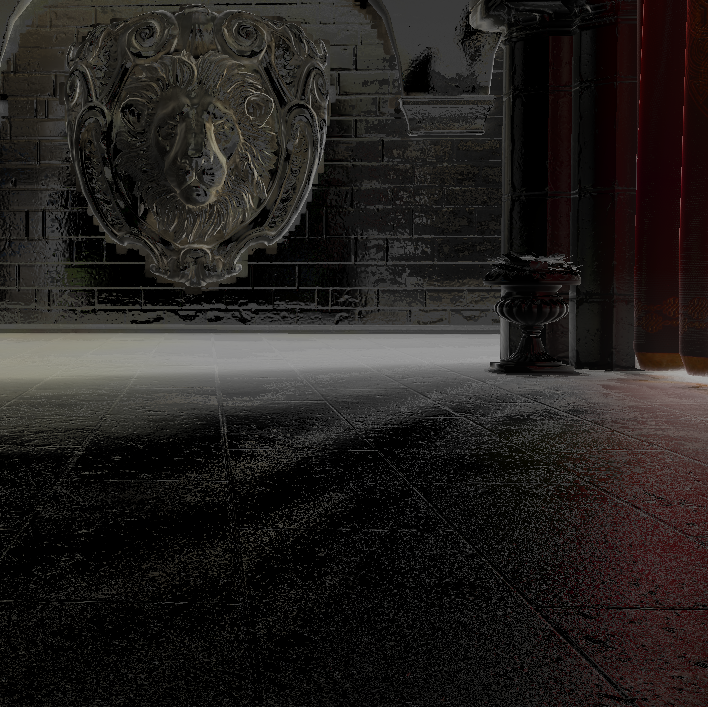
\includegraphics[width=1.0\linewidth]{images/banding.png}
\caption{\label{figure:banding}A screenshot showing banding artefacts in the specular component.}{}
\end{figure}

\bibliographystyle{acmsiggraph}
\bibliography{references}

\end{document}

